% !TeX spellcheck = en_US
\chapter{Model-Based Policy Learning}
As mentioned before, model-based \ac{RL} v.1.5 algorithm (\secref{sec:modelbasedrl1.5}) is a \hlb{stochastic open-loop} algorithm. The agent does see the next state, but it doesn't able to reason about the fact that more information will be available and make use out it. It simply plans the whole action sequence at each time step and assumes that it has to commit to that complete action plan. This is, in most case, \hlr{sub-optimal}. This section describes the \hlb{closed-loop} case, implying the agent aware that it will be able to see the state feedback and act upon it. Thus, instead of a complete action plan, the output is now a policy $\pi(\textbf{a}_t | \textbf{s}_t)$.

\begin{itemize}
	\item Stochastic open-loop case:\quad $\left\{\begin{matrix*}[l]
		\displaystyle p_\theta(\textbf{s}_1, \dots, \textbf{s}_T | \textbf{a}_1, \dots, \textbf{a}_T) = p(\textbf{s}_1) \prod_{t=1}^T p(\textbf{s}_{t+1} | \textbf{s}_t, \textbf{a}_t)\\
		\displaystyle \textbf{a}_1, \dots, \textbf{a}_T = \underset{\textbf{a}_1, \dots, \textbf{a}_T}{\arg\max}\; \mathbb{E} \left[ \sum_t r(\textbf{s}_t, \textbf{a}_t) | \textbf{a}_1, \dots, \textbf{a}_T \right]
	\end{matrix*}\right.$
	\item Stochastic closed-loop case:\quad $\left\{ \begin{matrix*}[l]
		\displaystyle p(\textbf{s}_1, \textbf{a}_1, \dots, \textbf{s}_T, \textbf{a}_T) = p(\textbf{s}_1) \prod_{t=1}^T \pi(\textbf{a}_t | \textbf{s}_t) p(\textbf{s}_{t+1} | \textbf{s}_t, \textbf{a}_t)\\
		\displaystyle \pi = \underset{\pi}{\arg\max}\; \mathbb{E}_{\tau \sim p(\tau)} \left[ \sum_t r(\textbf{s}_t, \textbf{a}_t) \right]
	\end{matrix*} \right.$
\end{itemize}

For the above policy $\pi$, there are possibly different forms for it:
\begin{itemize}
	\item Neural net: \hlr{global policy}, which would tell us what to do regardless of the state the agent is in the whole state space.
	\item Time-varying linear $\textbf{K}_t \textbf{s}_t + \textbf{k}_t$: \hlr{local policy}, which would be simple but only sufficient around particular area of a known trajectory
\end{itemize}

\section{Model-based RL v.2.0}
\label{sec:model-based-rl-2.0}
\begin{center}
	\begin{tikzpicture}[recnode/.style={rectangle, draw=black!60, very thick, minimum size=7mm}]
		\node[recnode](a1){$\textbf{a}_t = \pi_\theta(\textbf{s}_t)$};
		\node[recnode](s1)[right=of a1]{$\textbf{s}_{t+1} = f(\textbf{s}_t, \textbf{a}_t)$};
		\node[recnode](a2)[right=of s1]{$\textbf{a}_t = \pi_\theta(\textbf{s}_t)$};
		\node[recnode](s2)[right=of a2]{$\textbf{s}_{t+1} = f(\textbf{s}_t, \textbf{a}_t)$};
		\node[recnode](r1)[above=of a1]{$r(\textbf{s}_t, \textbf{a}_t)$};
		\node[recnode](r2)[above=of a2]{$r(\textbf{s}_t, \textbf{a}_t)$};
		\draw[thick, -latex, transform canvas={yshift=-2.5pt}](a1.east) -- (s1.west);
		\draw[red, thick, latex-, transform canvas={yshift= 2.5pt}](a1.east) -- (s1.west) node[midway, above=.2cm]{backprop};
		\draw[thick, -latex, transform canvas={yshift=-2.5pt}](a2.east) -- (s2.west);
		\draw[red, thick, latex-, transform canvas={yshift= 2.5pt}](a2.east) -- (s2.west) node[midway, above=.2cm]{backprop};
		\draw[thick, -latex, transform canvas={yshift=-2.5pt}](s1.east) -- (a2.west);
		\draw[red, thick, latex-, transform canvas={yshift= 2.5pt}](s1.east) -- (a2.west) node[midway, above=.2cm]{backprop};
		\draw[red, thick, -latex, transform canvas={xshift= 4.5pt}](r1.south) -- (a1.north);
		\draw[thick, latex-, transform canvas={xshift=-4.5pt}](r1.south) -- (a1.north);
		\draw[red, thick, -latex, transform canvas={xshift= 4.5pt}](r2.south) -- (a2.north);
		\draw[thick, latex-, transform canvas={xshift=-4.5pt}](r2.south) -- (a2.north);
	\end{tikzpicture}
\end{center}
\begin{enumerate}
	\item Run based policy $\pi_0(\textbf{a}_t, \textbf{s}_t)$ to collect $\mathcal{D} = \{ (\textbf{s, a, s'})_i \}$
	\item \tikzmark{mbrlv22}Learn dynamic model $f(\textbf{s,a})$ to minimize $\sum_{i} || f(\textbf{s}_{i}, \textbf{a}_{i}) - \textbf{s}_{i}' ||^2$
	\item Back-propagate through $f(\textbf{s,a})$ into the policy to optimize $\pi_\theta(\textbf{a}_t, \textbf{s}_t)$
	\item \tikzmark{mbrlv24}Run $\pi_\theta(\textbf{a}_t, \textbf{s}_t)$, appending the tuples $(\textbf{s, a, s'})$ to $\mathcal{D}$
	\begin{tikzpicture}[overlay,remember picture]
		\draw[very thick, -latex]
		([xshift=-7mm,yshift=1mm]pic cs:mbrlv24) --++ (-.5,0) |-
		([xshift=-7mm,yshift=1mm]pic cs:mbrlv22);
	\end{tikzpicture}
\end{enumerate}

\hlb{Problem:}
\begin{itemize}
	\item Similar parameter sensitivity problems as shooting methods\\
	The first action is way more important the the later ones.
	\item Similar problems to training long \ac{RNN}s with \ac{BPTT}\\
	Vanishing and exploding \ gradients
\end{itemize}

$\Rightarrow$ \hlb{Solutions:}
\begin{itemize}
	\item Use derivative-free ("model-free") planning algorithms with the model used to generate synthetic samples\\
	\Eg: Policy gradients has high variance, which can be reduced with lots of data, which can be generated by learned model
	\item Use simpler policies than neural nets
	\begin{itemize}
		\item \ac{LQR} with learned models (\ac{LQR}-\ac{FLM})
		\item Train \textbf{local} policies to solve simple tasks
		\item Combine them into \textbf{global} policies via supervised learning
	\end{itemize}
\end{itemize}

\section{Model-Free Learning With a Model}
This is one of the solutions for Model-based \ac{RL} v.2.0 (\secref{sec:model-based-rl-2.0}): use the learned model to generate synthetic data for "model-free" \ac{RL} algorithms, \eg, policy gradient. \cite{parmas2018icml}

\hlb{"Classic" Dyna} \cite{sutton1990integrated}: online Q-learning \ac{algor} that performs model-free \ac{RL} with a model
\begin{enumerate}
	\item Given state $s$, pick action $a$ using exploration policy
	\item Observe $s'$ and $r$, to get transition $(s, a, s', r)$
	\item Update model $\widehat{p}(s'|s,a)$ and $\widehat{r}(s,a)$ using $(s,a,s')$
	\item Q-update: $Q(s,a) \leftarrow Q(s,a) + \alpha \mathbb{E}_{s', r} [r + \underset{a'}{\max} Q(s', a') - Q(s, a) ]$
	\item Repeat $K$ times:\\
	6. \tikzmark{dyna5}Sample $(s,a) \sim \mathcal{B}$ from buffer of past states and actions\\
	7. \tikzmark{dyna6}Q-update: $Q(s,a) \leftarrow Q(s,a) + \alpha \mathbb{E}_{s', r} [r + \underset{a'}{\max} Q(s', a') - Q(s, a) ]$
	\begin{tikzpicture}[overlay,remember picture]
		\draw[very thick, -latex]
		([xshift=-7mm,yshift=1mm]pic cs:dyna6) --++ (-.5,0) |-
		([xshift=-7mm,yshift=1mm]pic cs:dyna5);
	\end{tikzpicture}
\end{enumerate}

\hlb{General "Dyna-style" model-based \ac{RL}:}
\begin{enumerate}
	\item Collect some data, consisting of transitions $(\textbf{s, a, s'}, r)$ \hlr{(1-million steps)}
	\item Learn model $\widehat{p}(s'|s,a)$ (and optionally, $\widehat{r}(s,a)$)
	\item Repeat $K$ times:\\
	4. Sample $s \sim \mathcal{B}$ from buffer\\
	5. Choose action $a$ (from $\mathcal{B}$, from $\pi$, or random)\\
	6. Simulate $s' \sim\widehat{p}(s'|s,a)$ (and $r = \widehat{r}(s,a)$)\\
	7. Train on $(s, a, s', r)$ with model-free \ac{RL}\\
	8. (optional) Take $N$ more model-based steps
\end{enumerate}
The above approach is:
\[\begin{matrix*}[l]
	\color{Green}+ \text{only requires short (as few as one step) rollouts from model}\\
	\color{Green}+ \text{still sees diverse states}
\end{matrix*}\]
\hlb{Problem:} if your model is inaccurate (which always is), the longer we roll-out the model, the more these errors compound. This leads to distribution shift, either in the model or the policy. This is also why this is suited for mostly short rollouts of the model.
$\Rightarrow$ Not very nice for Policy Gradients, but is okay for value-based approaches, actor-critic, \etc.

\hlb{Note:}
\begin{itemize}
	\item In Classic Dyna, step 5 is to choose action from buffer
	\item This general procedure is the basis for:
	\begin{itemize}
		\item \ac{MBA} \cite{gu2016continuous}
		\item \ac{MVE} \cite{feinberg2018model}
		\item \ac{MBPO} \cite{janner2019trust}
	\end{itemize}
\end{itemize}

\section{Local Models}
This is the second solution for model-based \ac{RL} v.2.0 (\secref{sec:model-based-rl-2.0}): instead of using neural network, we use simple policies, which is time-varying linear controller, \ie, \ac{LQR}-\ac{FLM}.

In order to use \ac{LQR} (\secref{sec:lqr}), we need $\displaystyle\frac{df}{d\textbf{x}_t}, \frac{df}{d\textbf{u}_t}, \frac{dc}{d\textbf{x}_t}, \frac{dc}{d\textbf{u}_t}$, in which, knowing the model would give us $\displaystyle\frac{df}{d\textbf{x}_t}, \frac{df}{d\textbf{u}_t}$. If continuous system sufficiently smooth and initial state distribution quite tight $\Rightarrow$ do linearization regression at every time step

$\Rightarrow$ \hlb{Idea:} fit $\displaystyle\frac{df}{d\textbf{x}_t}$ and $\displaystyle\frac{df}{d\textbf{u}_t}$ around \hlb{current trajectory / policy}

\hlb{\ac{LQR}-\ac{FLM} Algorithm:}
\begin{enumerate}
	\item \tikzmark{lqr-flm1}Run $p(\textbf{u}_t | \textbf{x}_t)$ on robot, collect $\mathcal{D} = \{\tau_i\}$
	\item Fit dynamics $p(\textbf{x}_{t+1} | \textbf{x}_t, \textbf{u}_t)$
	\begin{align*}
		&p(\textbf{x}_{t+1} | \textbf{x}_t, \textbf{u}_t) = \mathcal{N}(f(\textbf{x}_t, \textbf{u}_t), \Sigma)\\
		&f(\textbf{x}_t, \textbf{u}_t) \approx \textbf{A}_t \textbf{x}_t + \textbf{B}_t \textbf{u}_t\\
		&\textbf{A}_t = \frac{df}{d\textbf{x}_t} \quad \textbf{B}_t = \frac{df}{d\textbf{u}_t}
	\end{align*}
	\item \tikzmark{lqr-flm3}Improve controller $p(\textbf{u}_t | \textbf{x}_t)$ (\ac{LQR})
	\begin{tikzpicture}[overlay,remember picture]
		\draw[very thick, -latex]
		([xshift=-7mm,yshift=1mm]pic cs:lqr-flm3) --++ (-.5,0) |-
		([xshift=-7mm,yshift=1mm]pic cs:lqr-flm1);
	\end{tikzpicture}
\end{enumerate}

\hlb{Which controller to run?} $p(\textbf{u}_t | \textbf{x}_t)$
\begin{itemize}
	\item Version 0.5: $p(\textbf{u}_t | \textbf{x}_t) = \delta(\textbf{u}_t = \widehat{\textbf{u}}_t)$ doesn't correct deviations or drift
	\item Version 1.0: $p(\textbf{u}_t | \textbf{x}_t) = \delta \textbf{u}_t = \textbf{K}_t (\textbf{x}_t - \widehat{\textbf{x}}_t) + \textbf{k}_t + \widehat{\textbf{u}}_t$\\
	Better, but a little too good. When fitting the dynamics, we need data to be a little bit cluster, but not too much. \hlr{Still need to be varied, for exploration and fitting.}
	\item Version 2.0: $p(\textbf{u}_t | \textbf{x}_t) = \mathcal{N}(\textbf{K}_t (\textbf{x}_t - \widehat{\textbf{x}}_t) + \textbf{k}_t + \widehat{\textbf{u}}_t, \Sigma_t)$\\
	Set $\Sigma_t = \textbf{Q}_{\textbf{u}_t, \textbf{u}_t}^{-1}$
\end{itemize}

\hlb{How to fit the dynamics?} $p(x_{t+1} | x_t, u_t)$ given $\{ (\textbf{x}_t, \textbf{u}_t, \textbf{x}_{t+1})_i \}$
\begin{itemize}
	\item Version 1.0: At each time step using linear regression
	\[ p(\textbf{x}_{t+1} | \textbf{x}_t, \textbf{u}_t) = \mathcal{N}(\textbf{A}_t \textbf{x}_t + \textbf{B}_t \textbf{u}_t + \textbf{c}, \textbf{N}_t); \quad \textbf{A}_t \approx \frac{df}{d\textbf{x}_t}; \textbf{B}_t \approx \frac{df}{d\textbf{u}_t} \]
	\hlb{Problems:} linear regression requires number of samples that scale with dimensional states
	\item Version 2.0: fit using Bayesian linear regression\\
	Use your favorite global model as prior\\
	$\Rightarrow$ Can get away with fewer samples
\end{itemize}

\hlb{How to stay close to old controller?}\\
We want to stay close around local region of trajectories where we have linearize to approximation\\
$\Rightarrow$ Keep \ac{KL} divergence small (between old and new trajectories) \cite{levine2014learning}
\begin{align}
	&p(\textbf{u}_t | \textbf{x}_t) = \mathcal{N}(\textbf{K}_t (\textbf{x}_t - \widehat{\textbf{x}}_t) + \textbf{k}_t + \widehat{\textbf{u}}_t, \Sigma_t) && \text{the controller}\\
	&p(\tau) = p(\textbf{x}_1) \prod_{t=1}^T p(\textbf{u}_t | \textbf{x}_t) p(\textbf{x}_{t+1} | \textbf{x}_t, \textbf{u}_t) && \text{the resulting trajectory}\\
	& D_{KL}(p(\tau) || \bar{p}(\tau)) \leq \epsilon && \text{constraint on \ac{KL} divergence}
\end{align}

\section{Guided Policy Search}
\label{sec:guided-policy-search}
This is the extension of local policies to global policies. However, the idea behind this, which is similar to distillation of ensemble (Sec. 5.8, \href{AI_notes.pdf}{AI notes}), is also important in other settings.

Given many local policies, we take the data from these local policies and treat them as expert's demonstrations and combine them into a global policy. The global policy can be learned as a neural net with supervised learning from these local data.

\hlb{Guided Policy Search Algorithm:} \cite{levine2016end}
\begin{enumerate}
	\item \tikzmark{gps1}Optimize each local policy $\pi_{LQR, i}(\textbf{u}_t | \textbf{x}_t)$ on initial state $\textbf{x}_{0, i}, \text{ \ac{wrt} } \widetilde{c}_{k,i}(\textbf{x}_t, \textbf{u}_t)$
	\item Use samples from step (1) to train $\pi_{\theta}(\textbf{u}_t|\textbf{x}_t)$ to mimic all $\pi_{LQR, i}(\textbf{u}_t | \textbf{x}_t)$
	\item \tikzmark{gps3}Update cost function $\widetilde{c}_{k+1,i}(\textbf{x}_t, \textbf{u}_t) = c(\textbf{x}_t, \textbf{u}_t) + \lambda_{k+1, i} \log\pi_{\theta}(\textbf{u}_t | \textbf{x}_t)$
	\begin{tikzpicture}[overlay,remember picture]
		\draw[very thick, -latex]
		([xshift=-7mm,yshift=1mm]pic cs:gps3) --++ (-.5,0) |-
		([xshift=-7mm,yshift=1mm]pic cs:gps1);
	\end{tikzpicture}
\end{enumerate}
in which, $i$ indexes the initial state and the local solution, $k$ the iteration, $\widetilde{c}_{k,i}(\textbf{x}_t, \textbf{u}_t)$ is the modified cost, including the task reward, and the \ac{KL} between $\pi_{LQR, i}$ and $\pi_{\theta}PP$

\begin{figure}[hbt!]
	\centering
	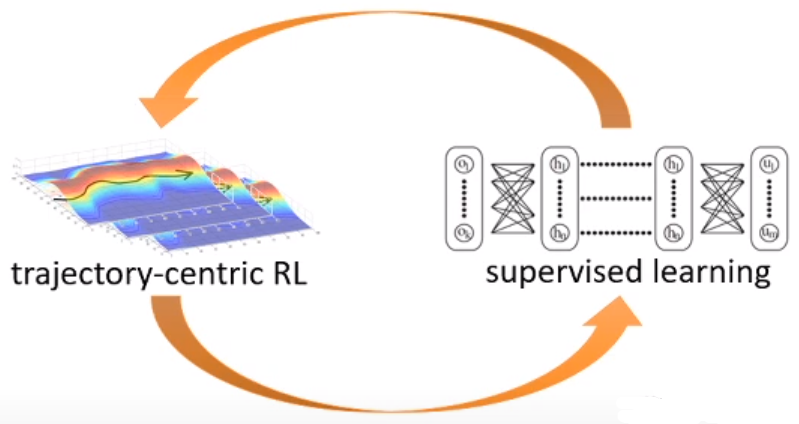
\includegraphics[width=.57\textwidth]{guided-policy-search.png}
	\caption{Guided policy search: algorithm sketch (\href{https://www.youtube.com/watch?v=DszxsbAl8Eo&list=PL_iWQOsE6TfURIIhCrlt-wj9ByIVpbfGc&index=55}{src}).}
\end{figure}

\hlb{Divide and Conquer \ac{RL} algorithm:}
\begin{enumerate}
	\item \tikzmark{dac1}Optimize each local policy $\pi_{\theta, i}(\textbf{u}_t | \textbf{x}_t)$ on initial state $\textbf{x}_{0, i}, \text{ \ac{wrt} } \widetilde{r}_{k,i}(\textbf{x}_t, \textbf{u}_t)$
	\item Use samples from step (1) to train $\pi_{\theta}(\textbf{u}_t|\textbf{x}_t)$ to mimic all $\pi_{\theta, i}(\textbf{u}_t | \textbf{x}_t)$
	\item \tikzmark{dac3}Update cost function $\widetilde{r}_{k+1,i}(\textbf{x}_t, \textbf{u}_t) = r(\textbf{x}_t, \textbf{u}_t) + \lambda_{k+1, i} \log\pi_{\theta}(\textbf{u}_t | \textbf{x}_t)$
	\begin{tikzpicture}[overlay,remember picture]
		\draw[very thick, -latex]
		([xshift=-7mm,yshift=1mm]pic cs:dac3) --++ (-.5,0) |-
		([xshift=-7mm,yshift=1mm]pic cs:dac1);
	\end{tikzpicture}
\end{enumerate}

\section{References}
\begin{itemize}
	\item \citeausm{levine2016end}. End-to-end training of deep visuomotor policies.
	\item \citeausm{rusu2015policy}. Policy distillation.
	\item \citeausm{parisotto2015actor}. Actor-mimic: Deep multitask and transfer reinforcement learning.
	\item \citeausm{ghosh2017divide}. Divide-and-conquer reinforcement learning.
	\item \citeausm{teh2017distral}. Distral: Robust multitask reinforcement learning.
\end{itemize}